\section{Esperimenti}

\subsection{Dataset}

Per gli esperimenti è stato utilizzato un dataset che contiene un totale di 12 dispositivi, che includono smartphone e tablet, di diverse case produttrici e modelli. In particolare i modelli in nostro possesso sono: un Galaxy S3, due Galaxy S3 mini, un Galaxy S4 mini, un Galaxy Tab 3, un Galaxy Tab, un Galaxy Trend Plus, un Huawei G6, un Ipad 2, un Ipad mini, un Iphone 4S, un Iphone 5. Di tutti questi dispositivi siamo in possesso di immagini direttamente acquisite (immagini naturali) e delle stesse immagini ma caricate e scaricate da Facebook.

La fase di estrazione delle fingerprints è stata eseguita tre volte con tre diversi sottoinsieme del dataset di dimensioni differenti. In particolare, seguendo gli esperimenti di \cite{ Amerini2014831} sono stati usati insiemi da 6 dispositivi (un Galaxy S3, due Galaxy S3 mini, un Galaxy S4 mini, un Galaxy Tab 3, un Galaxy Tab), 5 dispositivi (un Huawei G6, un Ipad 2, un Ipad mini, un Iphone 4S, un Iphone 5) e 4 dispositivi (un Galaxy Tab 3, un Galaxy Tab, un Galaxy Trend Plus, un Huawei G6). Dai dispositivi sono state selezionate 50 immagini, per un totale di 300, 250, 200 immagini rispettivamente per i tre casi.
Per il caso delle immagini scaricate da Facebook, oltre ai precedenti, sono stati eseguiti altri tre esperimenti aggiuntivi con un partizionamento diverso del dataset: sono stati usati insiemi da 6 dispositivi (un Galaxy Trend Plus, un Huawei G6, un Ipad 2, un Ipad mini, un Iphone 4S, un Iphone 5), 5 dispositivi (un Galaxy Tab 3, un Galaxy Tab, un Galaxy Trend Plus, un Huawei G6, un Ipad 2) e 4 dispositivi (un Ipad 2, un Ipad mini, un Iphone 4S, un Iphone 5).

Come spiegato in precedenza, la fase di validazione consiste nel verificare se sono state calcolate delle buone fingerprints, ovvero che siano in grado, data una generica immagine appartenente al dataset non usata in precedenza, di assegnarle al dispositivo corretto. In questa fase le camere sono state suddivise in gruppi uguali alla fase di estrazione delle fingerprint, utilizzando però 20 immagini da ciascun dispositivo non usate nella fase precedente.

\subsection{Risultati}

I risultati sono diversi per il caso delle immagini naturali e per il caso delle immagini di Facebook in alta risoluzione. Tali risultati sono ottenuti utilizzando le modalità descritte in precedenza, ovvero Normalized Cuts con $Ncuts$ come condizione di stop con soglia pari a $10^{-5}$ per il caso delle immagini direttamente acquisite dal dispositivo e con sogli pari a $4*10^{-5}$ per il caso della immagini caricate e poi scaricate da Facebook.

\begin{table}[ht]
\caption{Accuratezza del clustering}
\centering % used for centering table
\begin{tabular}{l c c c} % centered columns (4 columns)
\hline\hline %inserts double horizontal lines
Caso & Clusters & TPR & FPR \\ [0.5ex] % inserts table
%heading
\hline % inserts single horizontal line
Natural images (4) & 5 & 0.800 & 0.000 \\ % inserting body of the table
Natural images (5) & 7 & 0.714 & 0.000 \\
Natural images (6) & 8 & 0.750 & 0.000 \\
Facebook highres images (4) & 12 & 0.294 & 0.004 \\
Facebook highres images (5) & 12 & 0.333 & $10^{-5}$ \\
Facebook highres images (6) & 20 & 0.298 & $10^{-4}$ \\ [1ex] % [1ex] adds vertical space
\hline %inserts single line
\end{tabular}
\label{table:nonlin} % is used to refer this table in the text
\end{table}

Innanzitutto mostriamo in Tab.(1) i valori di TPR e FPR ottenuti dal clustering, con il relativo numero di clusters ottenuti, per gli esperimenti effettuati. Per quanto riguarda le immagini scaricate da Facebook, i valori mostrati sono la media dei due esperimenti che hanno lo stesso numero di dispositivi, ripartiti come spiegato in precedenza (tra parentesi è indicato i dispositivi considerati in ciascun esperimento).
Per il caso delle immagini naturali, i valori di FPR sono pari a zero, quindi ottimali, in quanto andranno a generare fingerprints pulite poichè i clusters conterranno solo immagini simili fra di loro.
Per il caso delle immagini scaricate da Facebook, i valori di FPR sono prossimi allo zero ma con una TPR media più bassa rispetto al caso precedente. Ciò implica che nei clusters ottenuti sarà presente una quantità trascurabile di falsi positivi e al contempo che il dataset è stato maggiormente partizionato. I clusters ottenuti, seppur puliti, conterranno meno immagini e quindi la fingerprint calcolata potrebbe risultare meno discriminante.

\begin{figure}[h]
\begin{center}
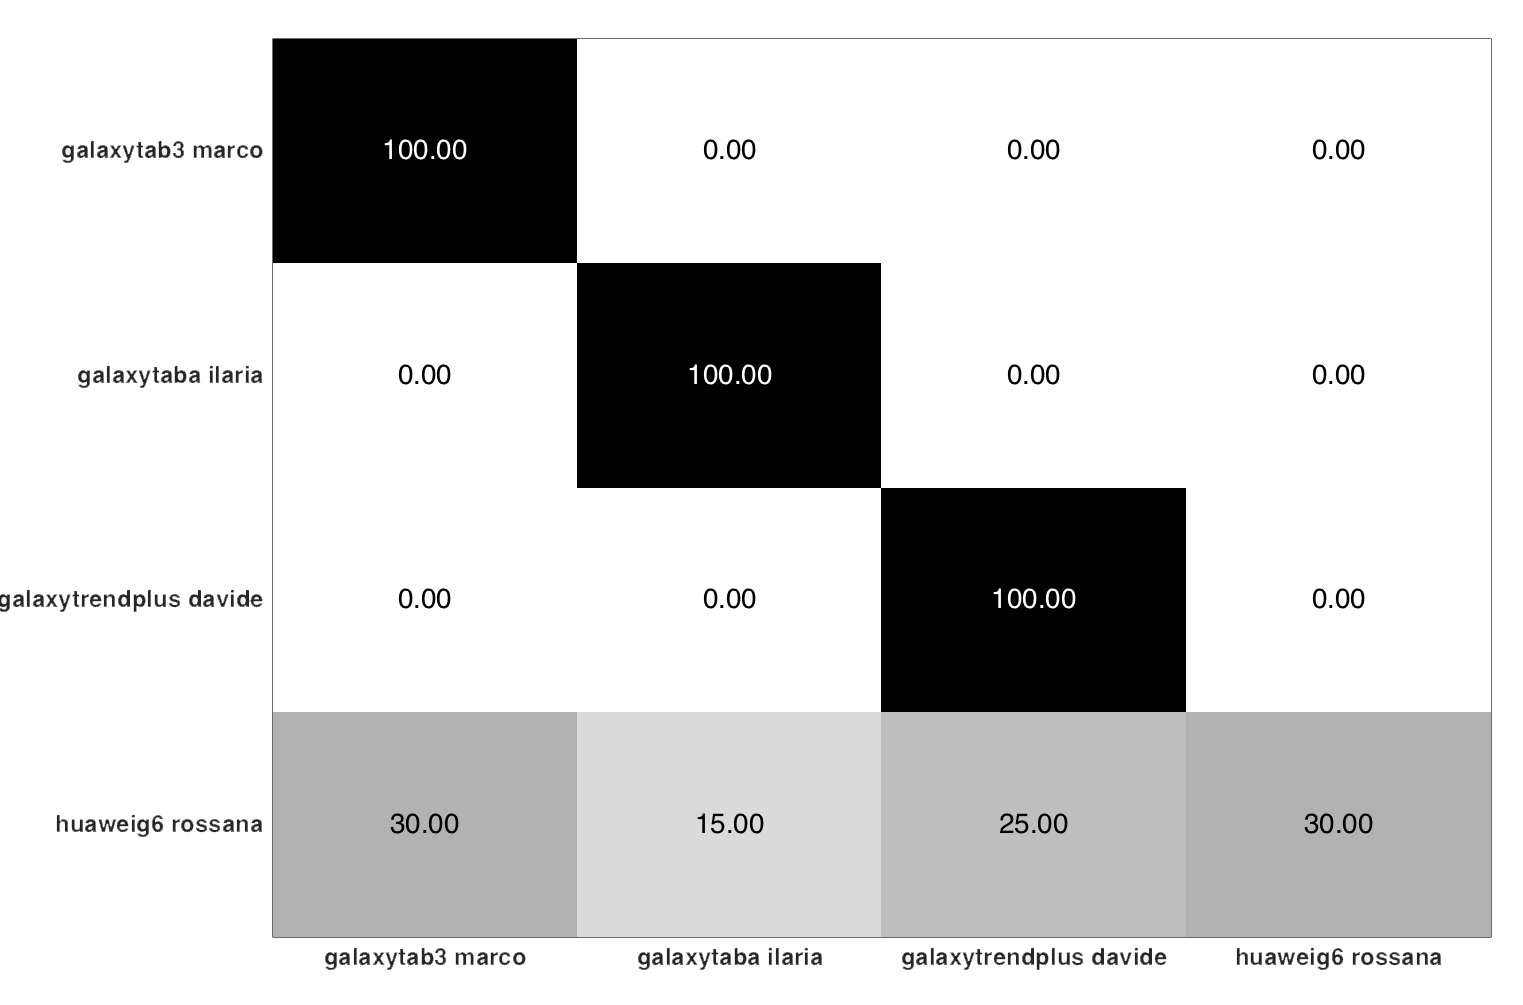
\includegraphics[width=0.45\textwidth]{images/confusionmatrix_nat_4.png}
\end{center}
  \caption{Matrice di confusione per il caso delle immagini naturali usando 4 dispositivi.}
\label{fig:validation}
\end{figure}

\begin{figure}[h]
\begin{center}
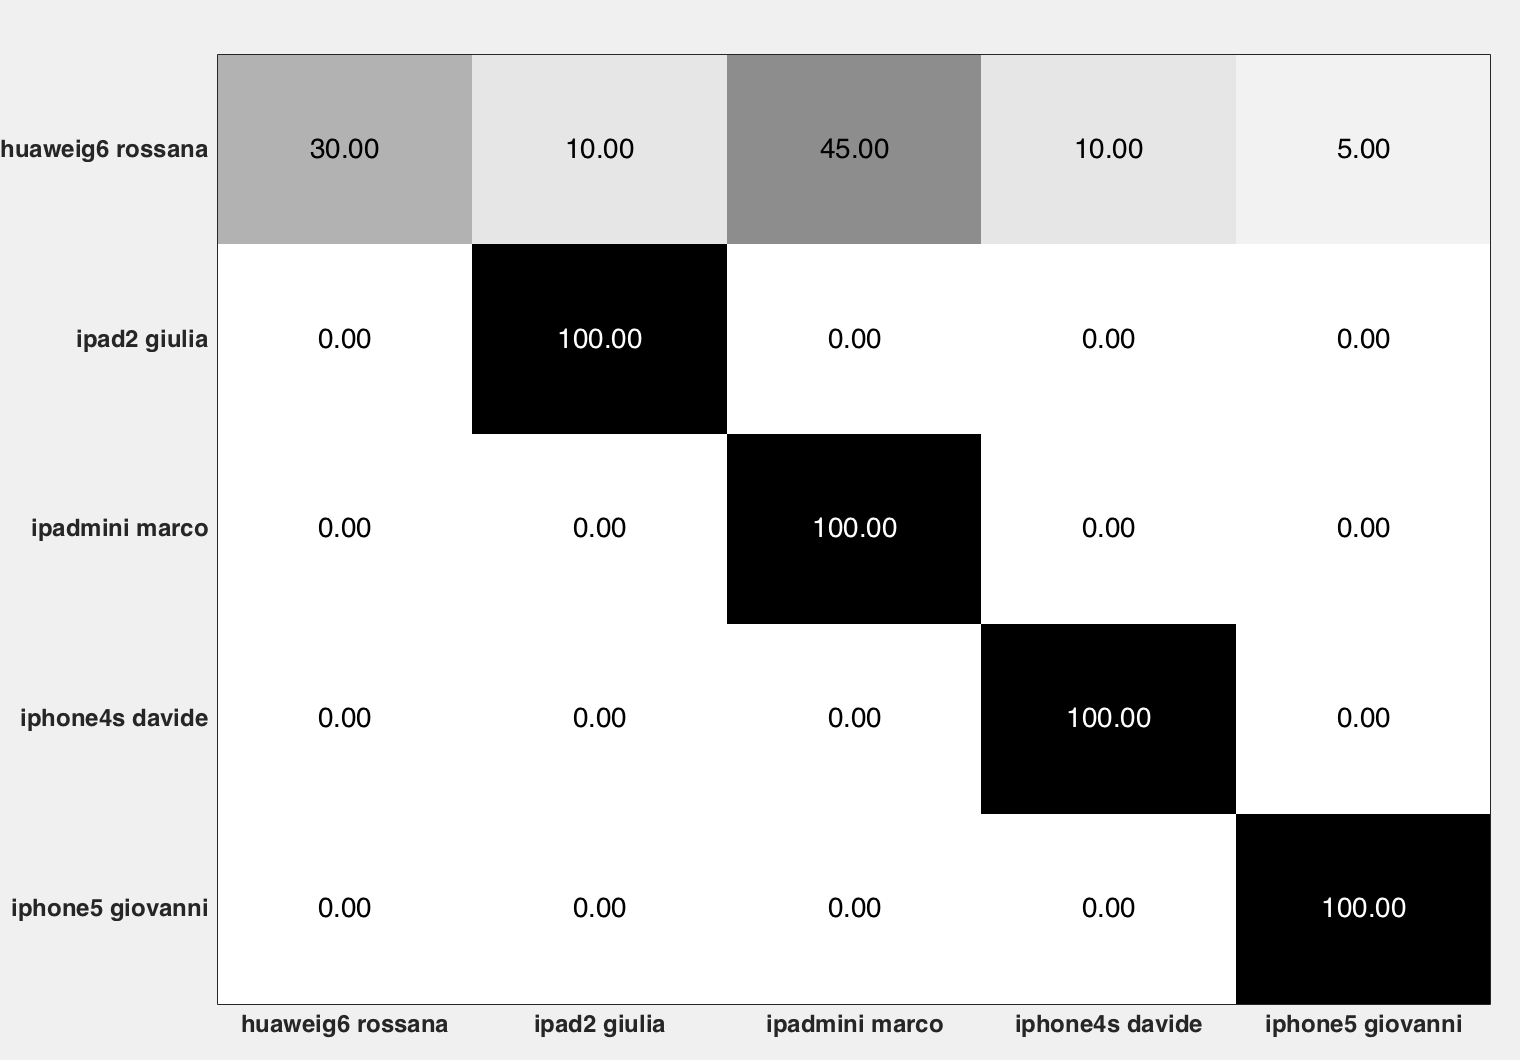
\includegraphics[width=0.45\textwidth]{images/confusionmatrix_nat_5.png}
\end{center}
  \caption{Matrice di confusione per il caso delle immagini naturali usando 5 dispositivi.}
\label{fig:validation}
\end{figure}

\begin{figure}[h]
\begin{center}
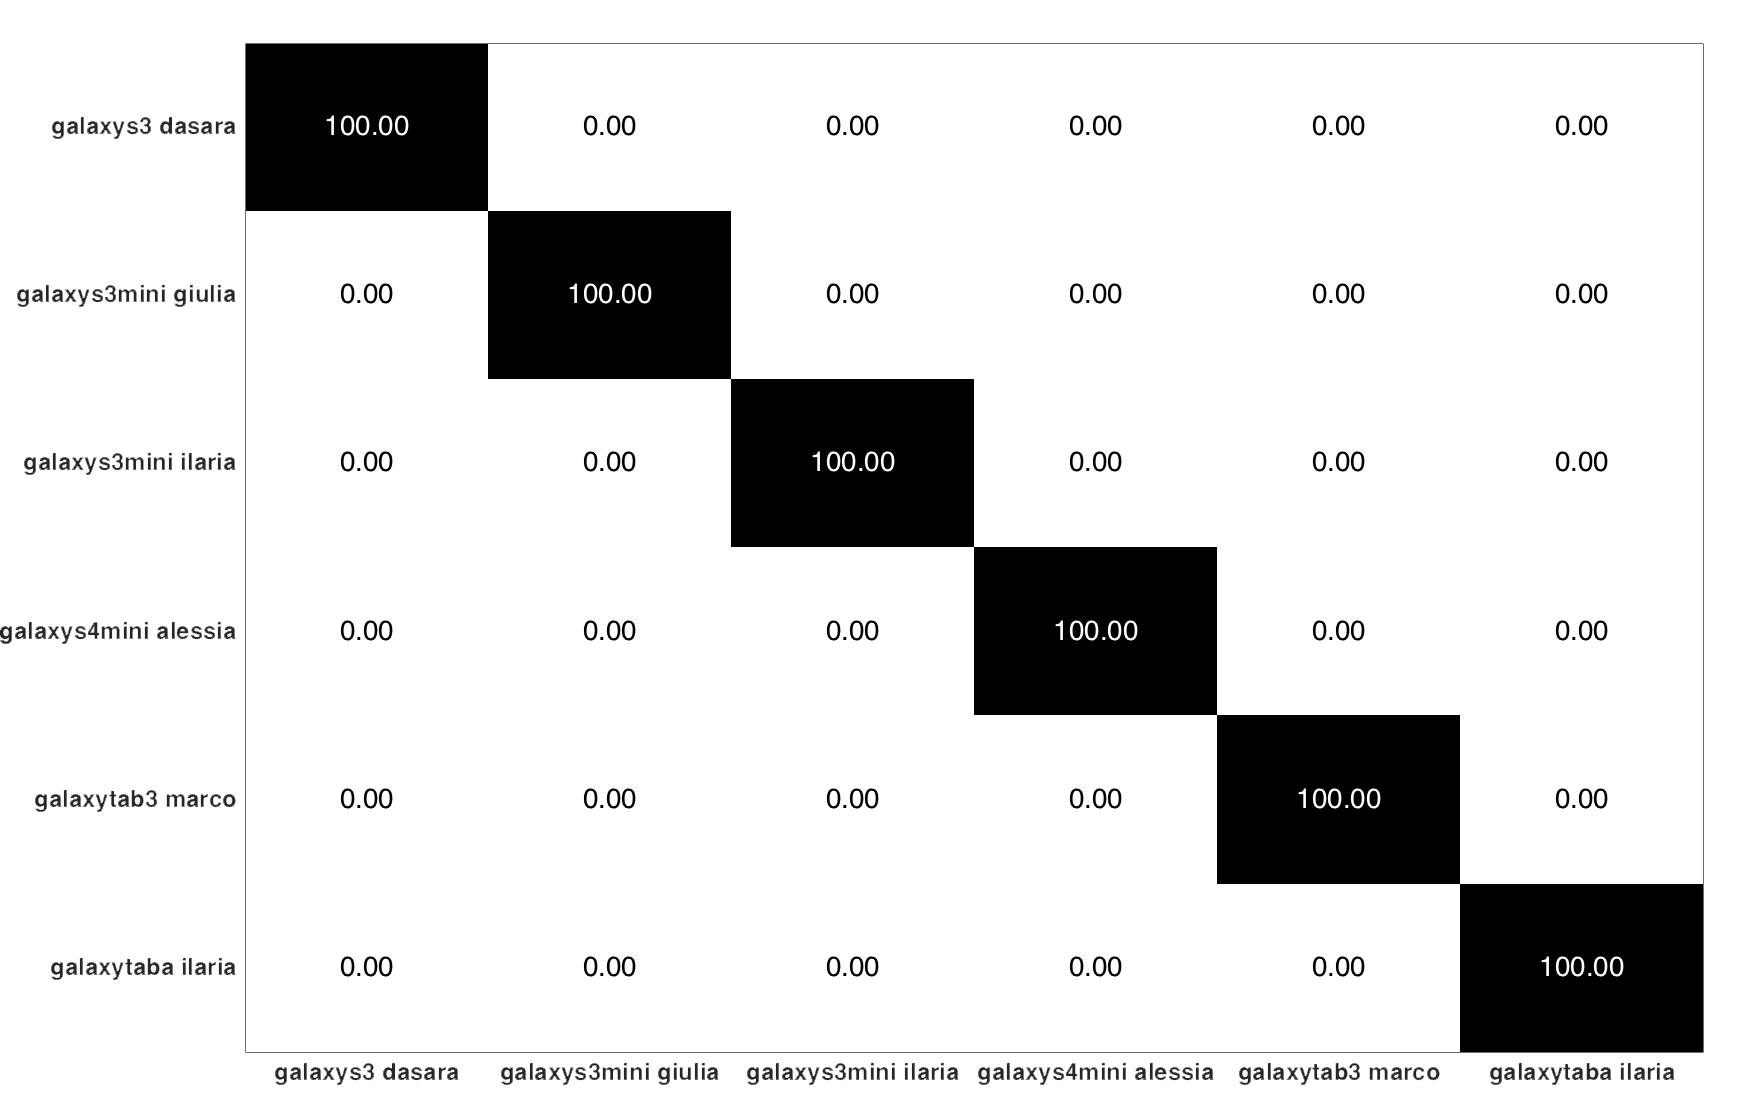
\includegraphics[width=0.45\textwidth]{images/confusionmatrix_nat_6.png}
\end{center}
  \caption{Matrice di confusione per il caso delle immagini naturali usando 6 dispositivi.}
\label{fig:validation}
\end{figure}

Nel caso delle immagini naturali la validazione ottiene dei buoni risultati rispetto a tutte e tre le ripartizioni del dataset. Le immagini di validazione vengono associate alla giusta fingerprint con un'accuratezza del 100\% su tutti i dispositivi; l'unica eccezione è rappresentata dal dispositivo Huawei G6. Gli errori in questo caso non sono però dovuti ad una fingerprint rumorosa, poichè nella fase di clustering è stata ottenuta una percentuale di falsi positivi pari a 0. L'errore di classificazione è quindi dovuto in fase di validazione, ovvero quando, utilizzando la PCE viene calcolata la similitudine fra le immagini di test e le fingerprint estratte.

\begin{figure}[h]
\begin{center}
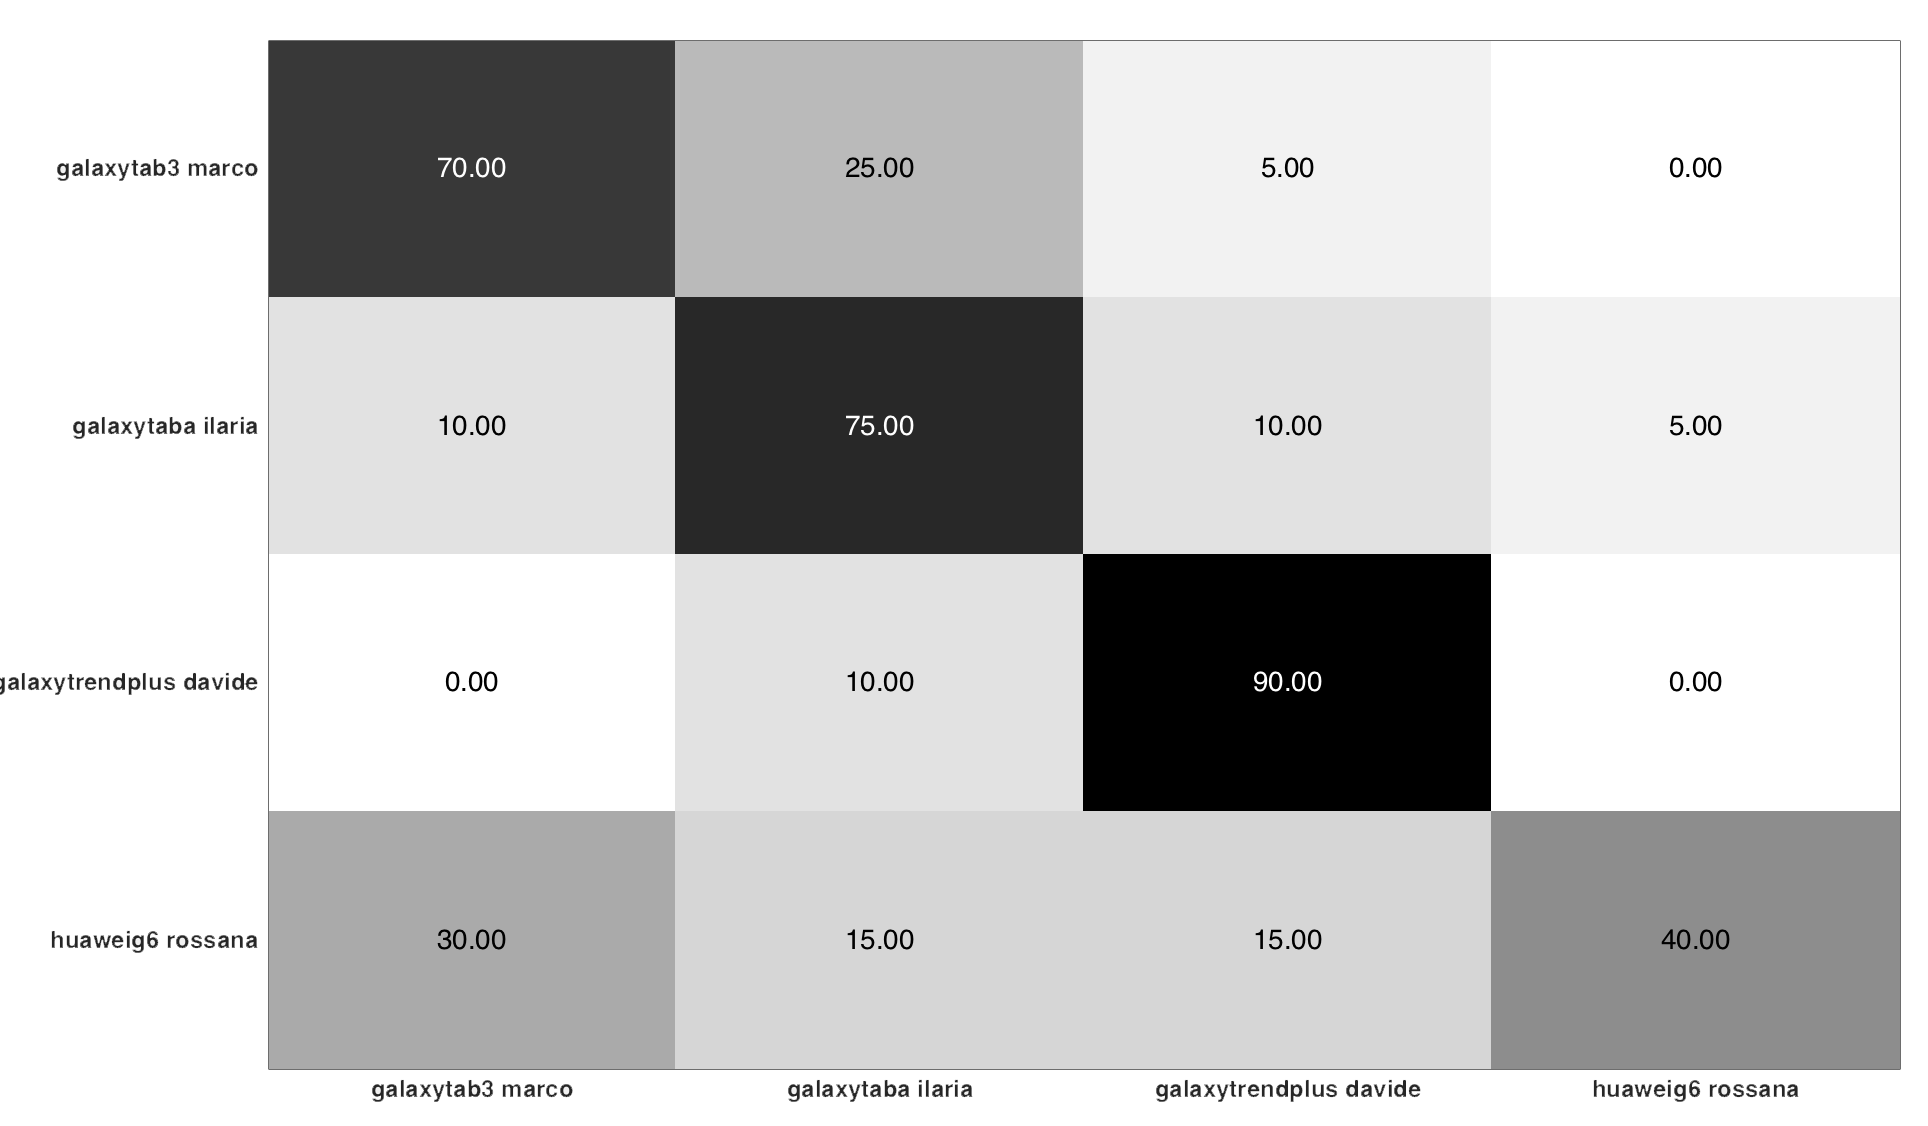
\includegraphics[width=0.45\textwidth]{images/confusion_matrix_fb_highres_4.png}
\end{center}
  \caption{Matrice di confusione per il caso delle immagini scaricate da Facebook usando gli stessi 4 dispositivi del caso delle immagini naturali. }
\label{fig:validation}
\end{figure}

\begin{figure}[h]
\begin{center}
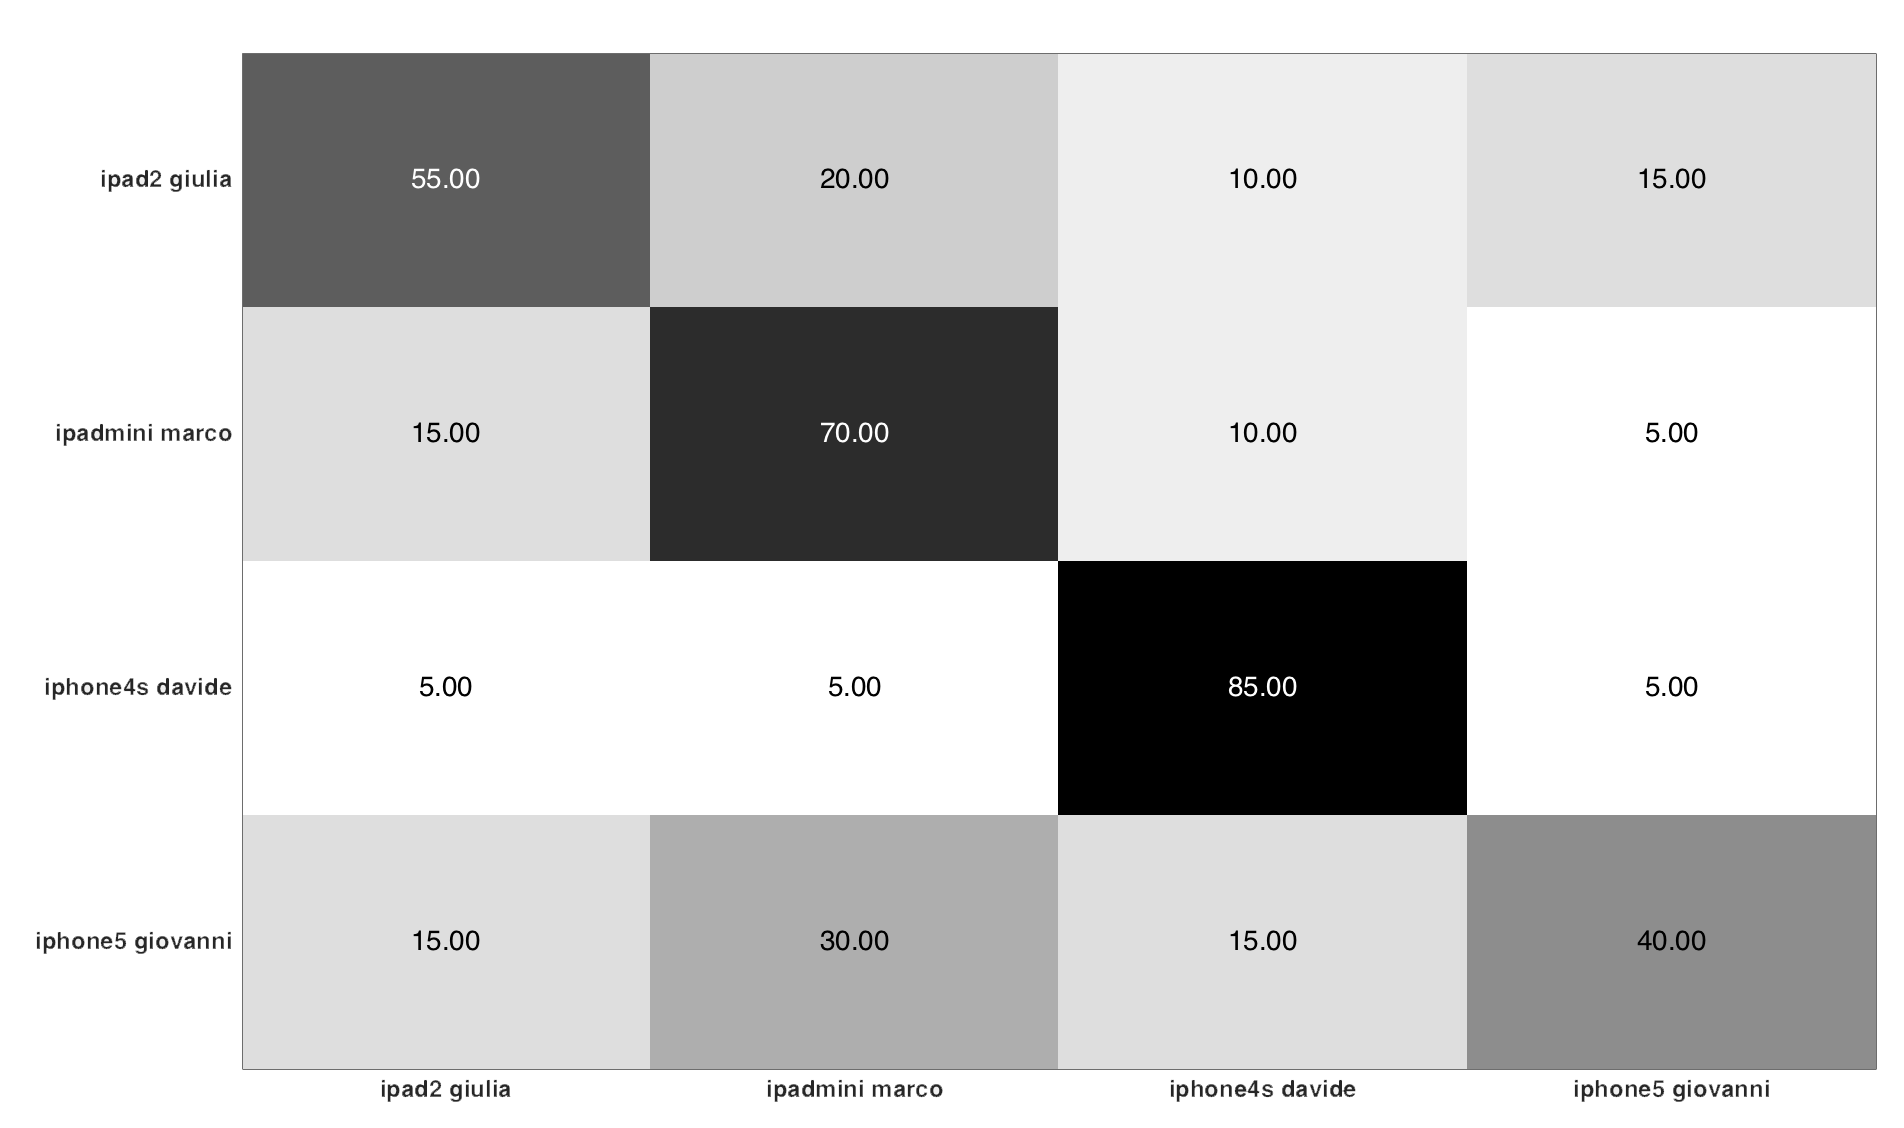
\includegraphics[width=0.45\textwidth]{images/confusion_matrix_fb_highres_4_bis.png}
\end{center}
  \caption{Matrice di confusione per il caso delle immagini scaricate da Facebook usando altri 4 dispositivi rispetto al caso delle immagini naturali. }
\label{fig:validation}
\end{figure}

\begin{figure}[h]
\begin{center}
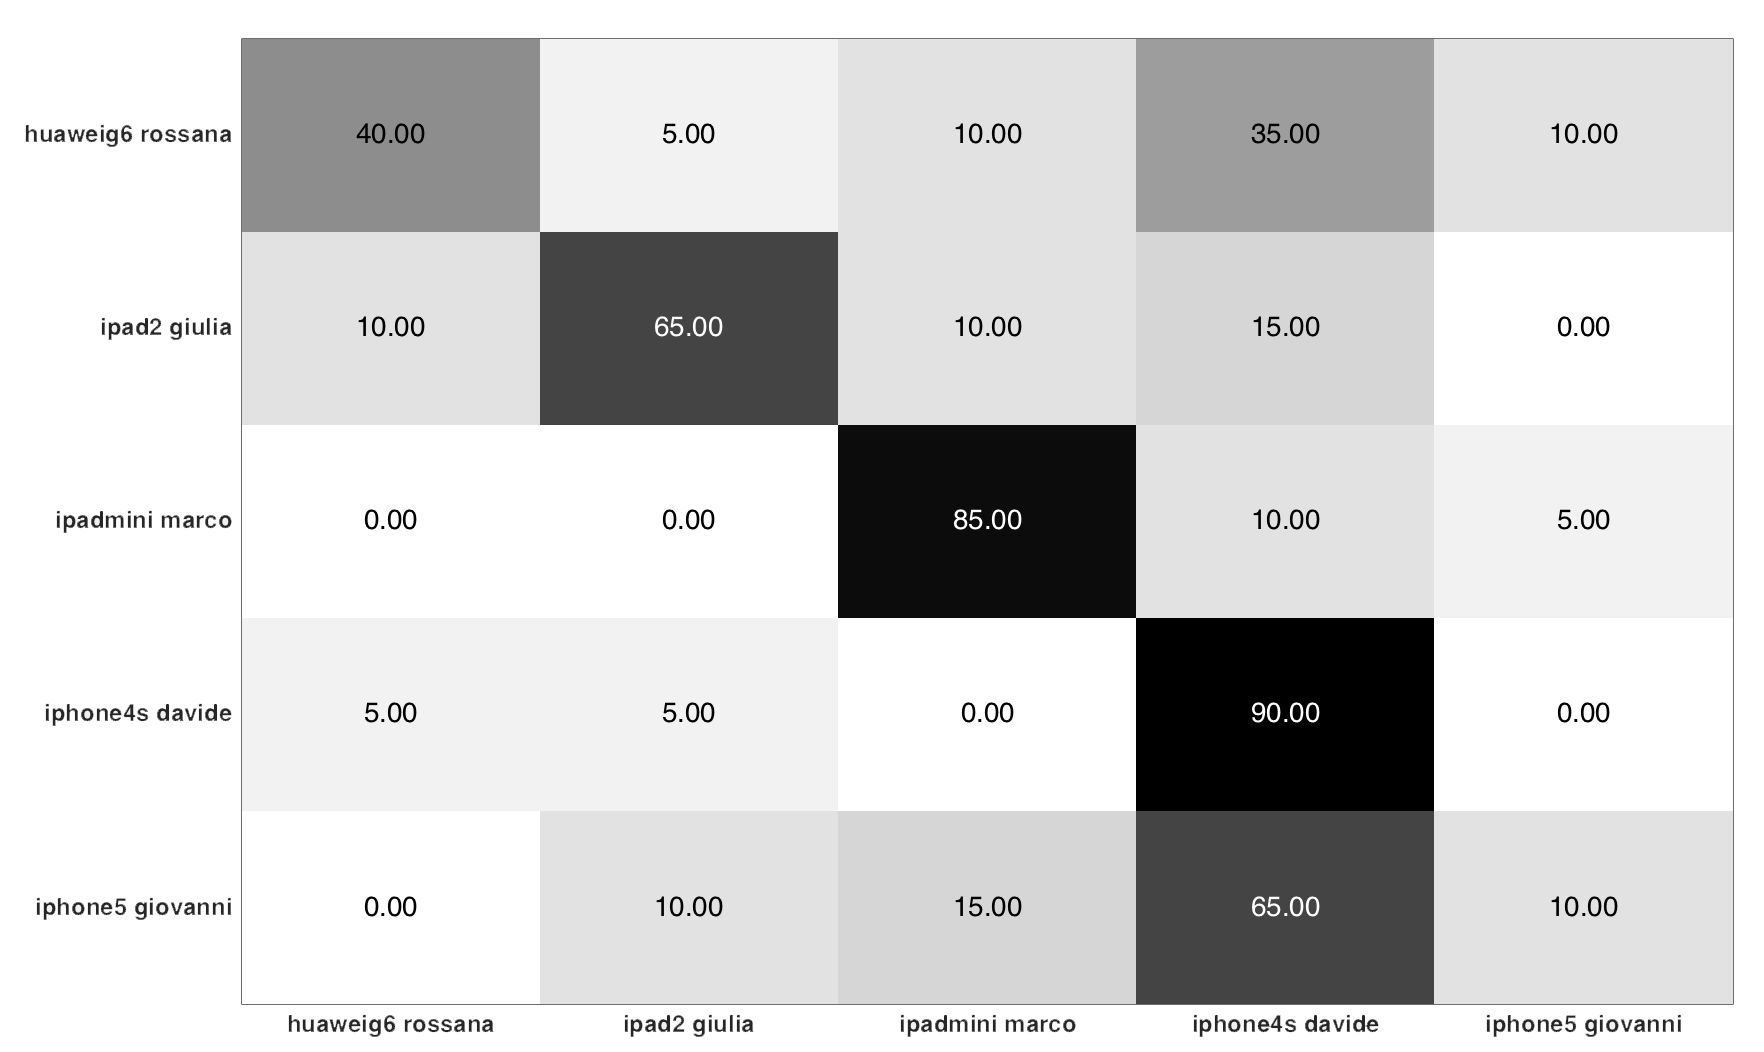
\includegraphics[width=0.45\textwidth]{images/confusion_matrix_fb_highres_5.png}
\end{center}
  \caption{Matrice di confusione per il caso delle immagini scaricate da Facebook usando gli stessi 5 dispositivi del caso delle immagini naturali.}
\label{fig:validation}
\end{figure}

\begin{figure}[h]
\begin{center}
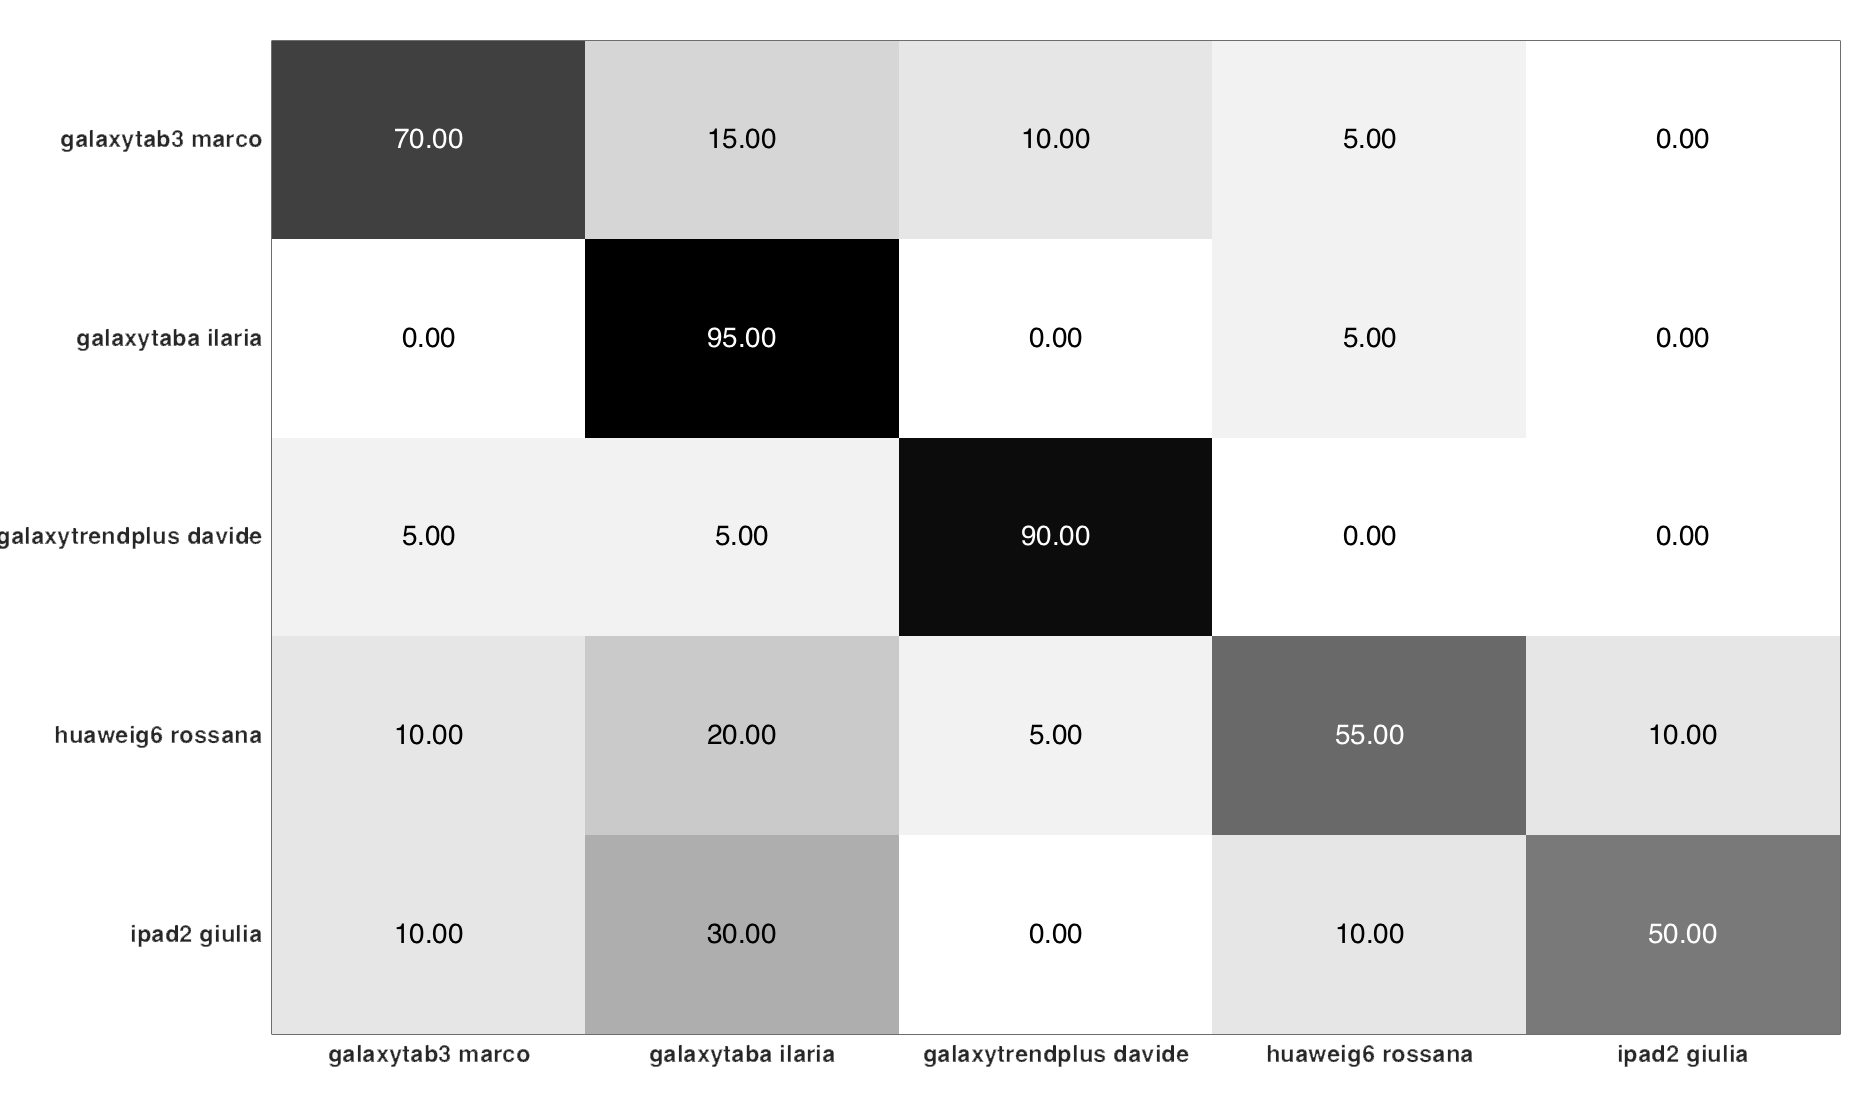
\includegraphics[width=0.45\textwidth]{images/confusion_matrix_fb_highres_5_bis.png}
\end{center}
  \caption{Matrice di confusione per il caso delle immagini scaricate da Facebook usando altri 5 dispositivi rispetto al caso delle immagini naturali. }
\label{fig:validation}
\end{figure}

\begin{figure}[h]
\begin{center}
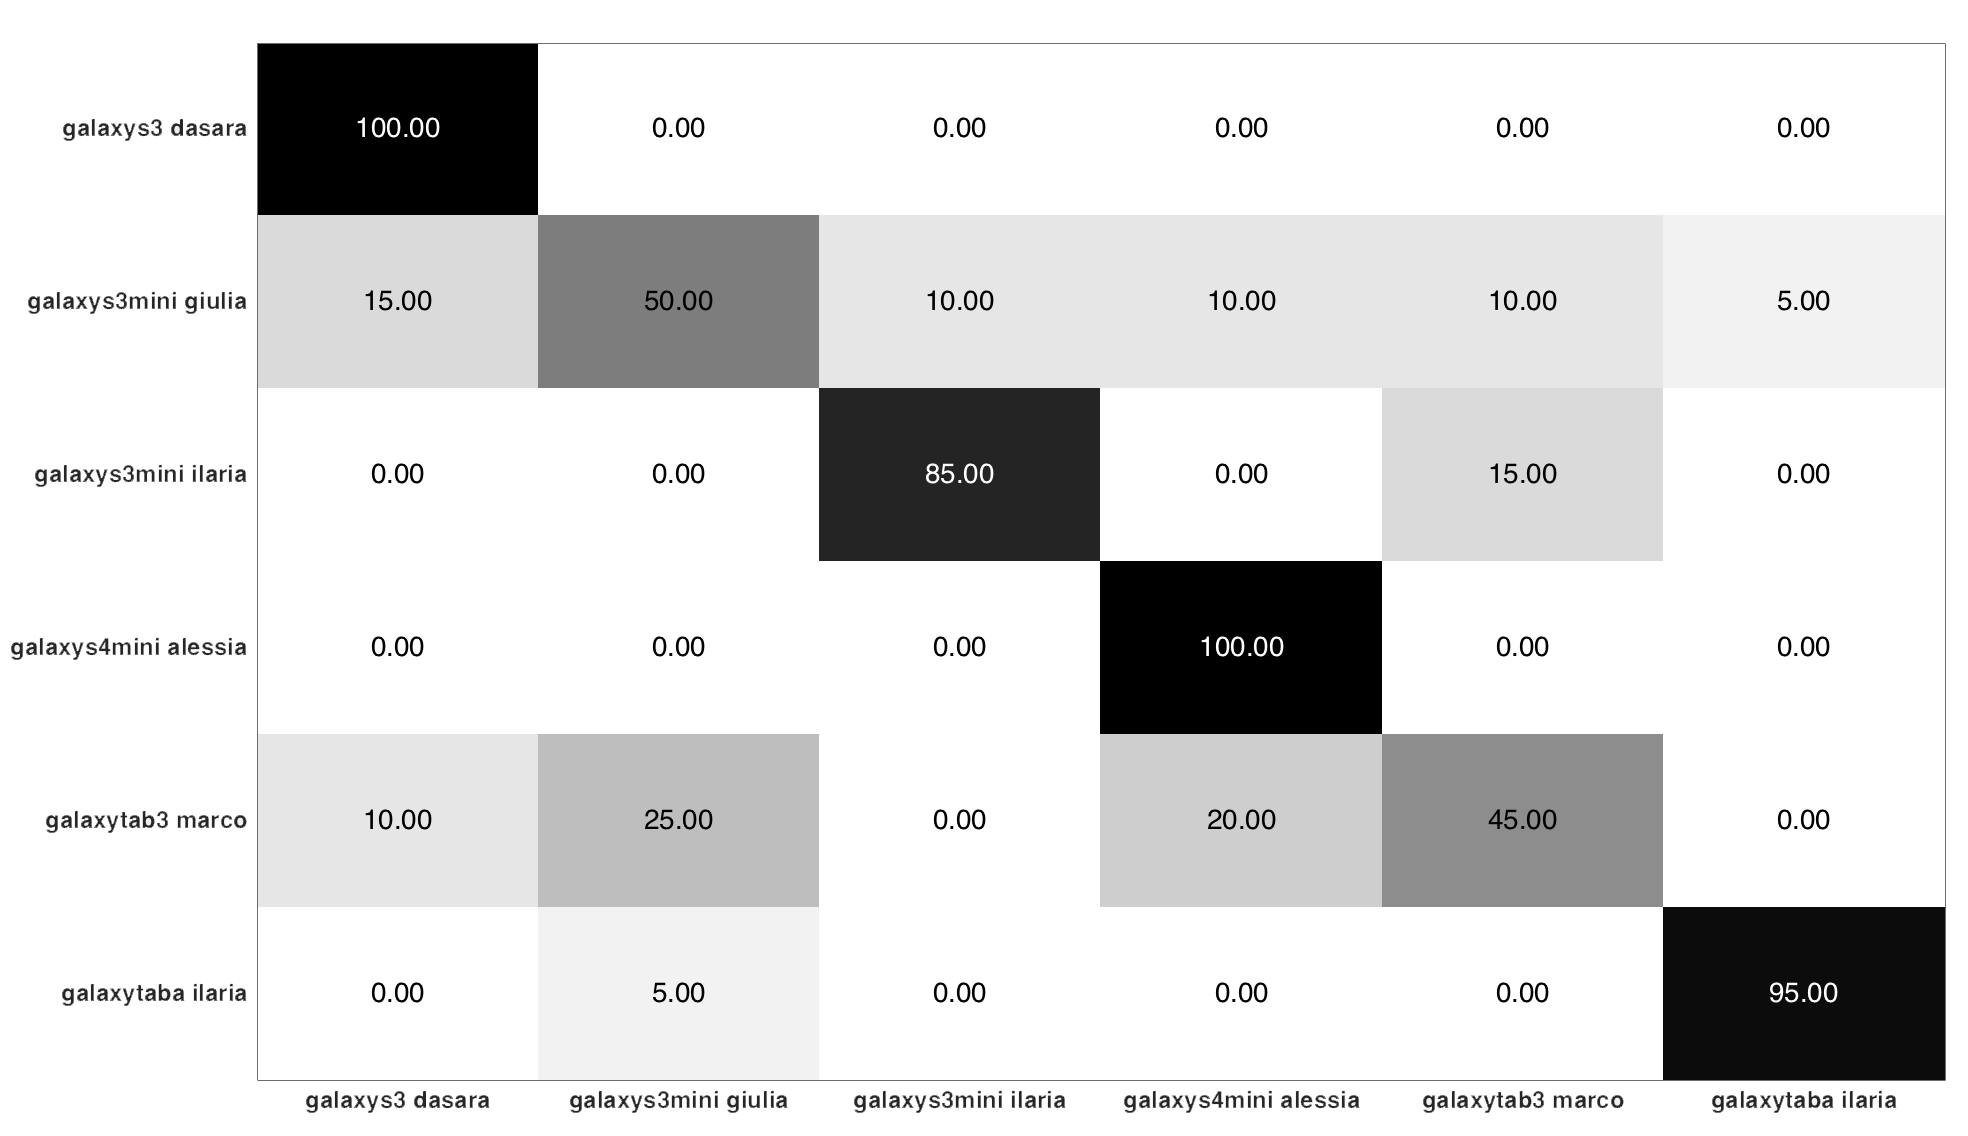
\includegraphics[width=0.45\textwidth]{images/confusion_matrix_fb_highres_6.png}
\end{center}
  \caption{Matrice di confusione per il caso delle immagini scaricate da Facebook usando gli stessi 6 dispositivi del caso delle immagini naturali.}
\label{fig:validation}
\end{figure}

\begin{figure}[h]
\begin{center}
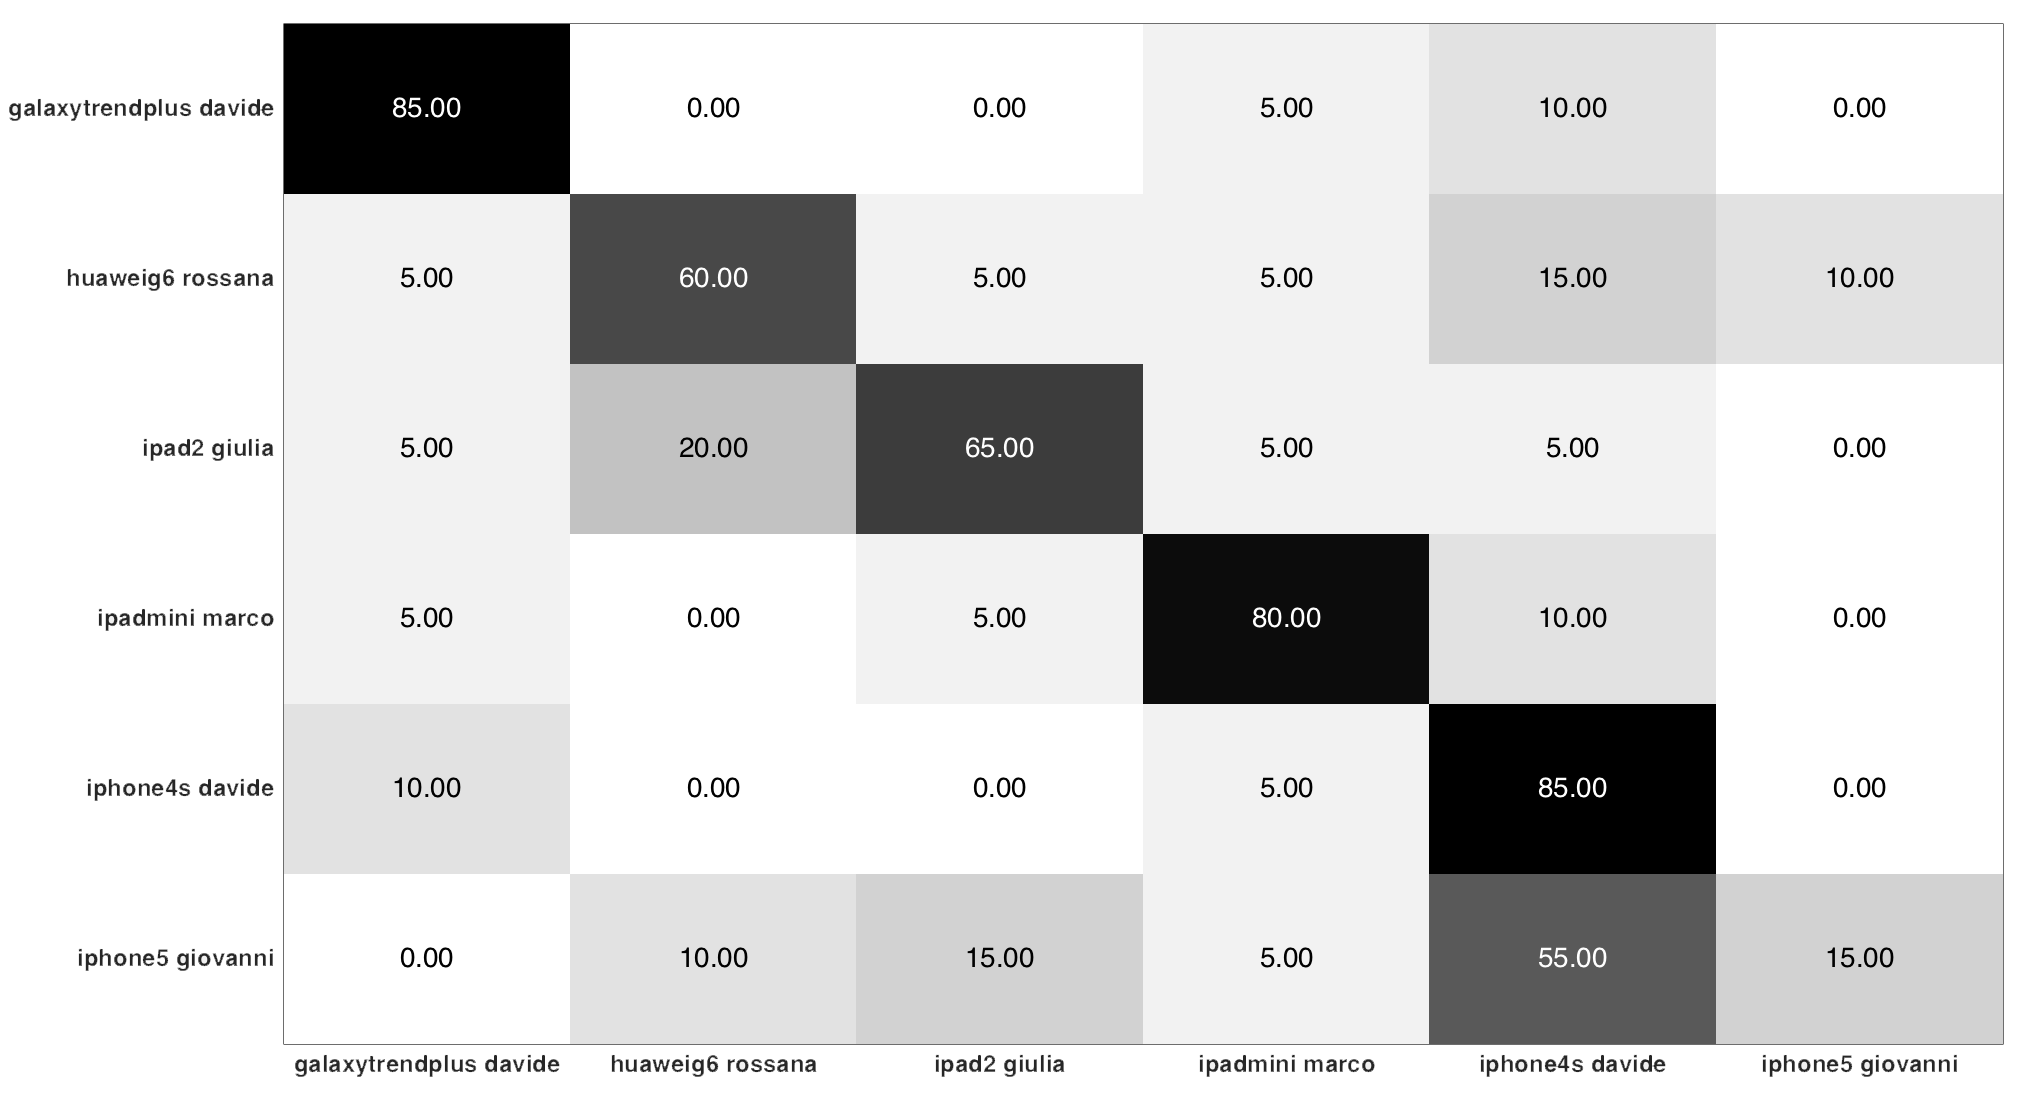
\includegraphics[width=0.45\textwidth]{images/confusion_matrix_fb_highres_6_bis.png}
\end{center}
  \caption{Matrice di confusione per il caso delle immagini scaricate da Facebook usando altri 6 dispositivi rispetto al caso delle immagini naturali. }
\label{fig:validation}
\end{figure}

Nel caso delle immagini scaricate da Facebook, i risultati sono leggermente differenti. La predizione della camera alterna risultati molto buoni, con un'accuratezza superiore al 85\% (i picchi massimi si toccano nella ripartizione da 6 dispositivi, con ben 3 camere con un'accuratezza superiore al 95\%), ad altri che invece hanno un'accuratezza intorno al 40-50\%. Confrontando in particolare le matrici di confusione degli esperimenti con i dataset in comune fra il caso delle immagini naturali e quello delle immagini di Facebook, è evidente che, pur usando lo stesso metodo, la predizione è meno precisa. Ciò è probabilmente dovuto al fatto che le immagini che vengono caricate su un social network, come detto in precedenza, subiscono una compressione che va ad incidere sulla capacità discriminante della PRNU e di conseguenza della PCE, utilizzata come misura di similarità, che otterrà valori all'incirca di un'ordine di grandezza inferiore rispetto alle immagini naturali. 
Anche in questo caso gli errori non sono dovuti al fatto che le fingerprints calcolate sono rumorose (avendo ottenuto una FPR prossima allo zero, queste sono in realtà pulite), quanto al fatto che la compressione causa i problemi detti in precedenza sulla PRNU e la PCE.
Da notare che sono sempre i soliti dispositivi ad ottenere le migliori prestazioni, indipendentemente dall'insieme di dispositivi in cui sono presenti nei vari esperimenti.

Si può dedurre dai risultati che il nostro metodo di identificazione automatica dei dispositivi è efficace nel caso delle immagini naturali, i risultati della validazione sono molto buoni ad eccezione di un unico dispositivo. Per quanto riguarda le immagini scaricate da Facebook, la predizione è meno precisa a causa della compressione subita. Tuttavia la compressione sembra incidere maggiormente alcuni dispositivi piuttosto che altri.